% Generated by Sphinx.
\def\sphinxdocclass{report}
\documentclass[letterpaper,10pt,spanish]{sphinxmanual}
\usepackage[utf8]{inputenc}
\DeclareUnicodeCharacter{00A0}{\nobreakspace}
\usepackage[T1]{fontenc}
\usepackage{babel}
\usepackage{times}
\usepackage[Sonny]{fncychap}
\usepackage{longtable}
\usepackage{sphinx}
\usepackage{multirow}


\title{Opinia Documentation}
\date{19 de November de 2012}
\release{1.0}
\author{Augusto Jair y Pedro Ludueña}
\newcommand{\sphinxlogo}{}
\renewcommand{\releasename}{Release}
\makeindex

\makeatletter
\def\PYG@reset{\let\PYG@it=\relax \let\PYG@bf=\relax%
    \let\PYG@ul=\relax \let\PYG@tc=\relax%
    \let\PYG@bc=\relax \let\PYG@ff=\relax}
\def\PYG@tok#1{\csname PYG@tok@#1\endcsname}
\def\PYG@toks#1+{\ifx\relax#1\empty\else%
    \PYG@tok{#1}\expandafter\PYG@toks\fi}
\def\PYG@do#1{\PYG@bc{\PYG@tc{\PYG@ul{%
    \PYG@it{\PYG@bf{\PYG@ff{#1}}}}}}}
\def\PYG#1#2{\PYG@reset\PYG@toks#1+\relax+\PYG@do{#2}}

\expandafter\def\csname PYG@tok@gd\endcsname{\def\PYG@tc##1{\textcolor[rgb]{0.63,0.00,0.00}{##1}}}
\expandafter\def\csname PYG@tok@gu\endcsname{\let\PYG@bf=\textbf\def\PYG@tc##1{\textcolor[rgb]{0.50,0.00,0.50}{##1}}}
\expandafter\def\csname PYG@tok@gt\endcsname{\def\PYG@tc##1{\textcolor[rgb]{0.00,0.25,0.82}{##1}}}
\expandafter\def\csname PYG@tok@gs\endcsname{\let\PYG@bf=\textbf}
\expandafter\def\csname PYG@tok@gr\endcsname{\def\PYG@tc##1{\textcolor[rgb]{1.00,0.00,0.00}{##1}}}
\expandafter\def\csname PYG@tok@cm\endcsname{\let\PYG@it=\textit\def\PYG@tc##1{\textcolor[rgb]{0.25,0.50,0.56}{##1}}}
\expandafter\def\csname PYG@tok@vg\endcsname{\def\PYG@tc##1{\textcolor[rgb]{0.73,0.38,0.84}{##1}}}
\expandafter\def\csname PYG@tok@m\endcsname{\def\PYG@tc##1{\textcolor[rgb]{0.13,0.50,0.31}{##1}}}
\expandafter\def\csname PYG@tok@mh\endcsname{\def\PYG@tc##1{\textcolor[rgb]{0.13,0.50,0.31}{##1}}}
\expandafter\def\csname PYG@tok@cs\endcsname{\def\PYG@tc##1{\textcolor[rgb]{0.25,0.50,0.56}{##1}}\def\PYG@bc##1{\setlength{\fboxsep}{0pt}\colorbox[rgb]{1.00,0.94,0.94}{\strut ##1}}}
\expandafter\def\csname PYG@tok@ge\endcsname{\let\PYG@it=\textit}
\expandafter\def\csname PYG@tok@vc\endcsname{\def\PYG@tc##1{\textcolor[rgb]{0.73,0.38,0.84}{##1}}}
\expandafter\def\csname PYG@tok@il\endcsname{\def\PYG@tc##1{\textcolor[rgb]{0.13,0.50,0.31}{##1}}}
\expandafter\def\csname PYG@tok@go\endcsname{\def\PYG@tc##1{\textcolor[rgb]{0.19,0.19,0.19}{##1}}}
\expandafter\def\csname PYG@tok@cp\endcsname{\def\PYG@tc##1{\textcolor[rgb]{0.00,0.44,0.13}{##1}}}
\expandafter\def\csname PYG@tok@gi\endcsname{\def\PYG@tc##1{\textcolor[rgb]{0.00,0.63,0.00}{##1}}}
\expandafter\def\csname PYG@tok@gh\endcsname{\let\PYG@bf=\textbf\def\PYG@tc##1{\textcolor[rgb]{0.00,0.00,0.50}{##1}}}
\expandafter\def\csname PYG@tok@ni\endcsname{\let\PYG@bf=\textbf\def\PYG@tc##1{\textcolor[rgb]{0.84,0.33,0.22}{##1}}}
\expandafter\def\csname PYG@tok@nl\endcsname{\let\PYG@bf=\textbf\def\PYG@tc##1{\textcolor[rgb]{0.00,0.13,0.44}{##1}}}
\expandafter\def\csname PYG@tok@nn\endcsname{\let\PYG@bf=\textbf\def\PYG@tc##1{\textcolor[rgb]{0.05,0.52,0.71}{##1}}}
\expandafter\def\csname PYG@tok@no\endcsname{\def\PYG@tc##1{\textcolor[rgb]{0.38,0.68,0.84}{##1}}}
\expandafter\def\csname PYG@tok@na\endcsname{\def\PYG@tc##1{\textcolor[rgb]{0.25,0.44,0.63}{##1}}}
\expandafter\def\csname PYG@tok@nb\endcsname{\def\PYG@tc##1{\textcolor[rgb]{0.00,0.44,0.13}{##1}}}
\expandafter\def\csname PYG@tok@nc\endcsname{\let\PYG@bf=\textbf\def\PYG@tc##1{\textcolor[rgb]{0.05,0.52,0.71}{##1}}}
\expandafter\def\csname PYG@tok@nd\endcsname{\let\PYG@bf=\textbf\def\PYG@tc##1{\textcolor[rgb]{0.33,0.33,0.33}{##1}}}
\expandafter\def\csname PYG@tok@ne\endcsname{\def\PYG@tc##1{\textcolor[rgb]{0.00,0.44,0.13}{##1}}}
\expandafter\def\csname PYG@tok@nf\endcsname{\def\PYG@tc##1{\textcolor[rgb]{0.02,0.16,0.49}{##1}}}
\expandafter\def\csname PYG@tok@si\endcsname{\let\PYG@it=\textit\def\PYG@tc##1{\textcolor[rgb]{0.44,0.63,0.82}{##1}}}
\expandafter\def\csname PYG@tok@s2\endcsname{\def\PYG@tc##1{\textcolor[rgb]{0.25,0.44,0.63}{##1}}}
\expandafter\def\csname PYG@tok@vi\endcsname{\def\PYG@tc##1{\textcolor[rgb]{0.73,0.38,0.84}{##1}}}
\expandafter\def\csname PYG@tok@nt\endcsname{\let\PYG@bf=\textbf\def\PYG@tc##1{\textcolor[rgb]{0.02,0.16,0.45}{##1}}}
\expandafter\def\csname PYG@tok@nv\endcsname{\def\PYG@tc##1{\textcolor[rgb]{0.73,0.38,0.84}{##1}}}
\expandafter\def\csname PYG@tok@s1\endcsname{\def\PYG@tc##1{\textcolor[rgb]{0.25,0.44,0.63}{##1}}}
\expandafter\def\csname PYG@tok@gp\endcsname{\let\PYG@bf=\textbf\def\PYG@tc##1{\textcolor[rgb]{0.78,0.36,0.04}{##1}}}
\expandafter\def\csname PYG@tok@sh\endcsname{\def\PYG@tc##1{\textcolor[rgb]{0.25,0.44,0.63}{##1}}}
\expandafter\def\csname PYG@tok@ow\endcsname{\let\PYG@bf=\textbf\def\PYG@tc##1{\textcolor[rgb]{0.00,0.44,0.13}{##1}}}
\expandafter\def\csname PYG@tok@sx\endcsname{\def\PYG@tc##1{\textcolor[rgb]{0.78,0.36,0.04}{##1}}}
\expandafter\def\csname PYG@tok@bp\endcsname{\def\PYG@tc##1{\textcolor[rgb]{0.00,0.44,0.13}{##1}}}
\expandafter\def\csname PYG@tok@c1\endcsname{\let\PYG@it=\textit\def\PYG@tc##1{\textcolor[rgb]{0.25,0.50,0.56}{##1}}}
\expandafter\def\csname PYG@tok@kc\endcsname{\let\PYG@bf=\textbf\def\PYG@tc##1{\textcolor[rgb]{0.00,0.44,0.13}{##1}}}
\expandafter\def\csname PYG@tok@c\endcsname{\let\PYG@it=\textit\def\PYG@tc##1{\textcolor[rgb]{0.25,0.50,0.56}{##1}}}
\expandafter\def\csname PYG@tok@mf\endcsname{\def\PYG@tc##1{\textcolor[rgb]{0.13,0.50,0.31}{##1}}}
\expandafter\def\csname PYG@tok@err\endcsname{\def\PYG@bc##1{\setlength{\fboxsep}{0pt}\fcolorbox[rgb]{1.00,0.00,0.00}{1,1,1}{\strut ##1}}}
\expandafter\def\csname PYG@tok@kd\endcsname{\let\PYG@bf=\textbf\def\PYG@tc##1{\textcolor[rgb]{0.00,0.44,0.13}{##1}}}
\expandafter\def\csname PYG@tok@ss\endcsname{\def\PYG@tc##1{\textcolor[rgb]{0.32,0.47,0.09}{##1}}}
\expandafter\def\csname PYG@tok@sr\endcsname{\def\PYG@tc##1{\textcolor[rgb]{0.14,0.33,0.53}{##1}}}
\expandafter\def\csname PYG@tok@mo\endcsname{\def\PYG@tc##1{\textcolor[rgb]{0.13,0.50,0.31}{##1}}}
\expandafter\def\csname PYG@tok@mi\endcsname{\def\PYG@tc##1{\textcolor[rgb]{0.13,0.50,0.31}{##1}}}
\expandafter\def\csname PYG@tok@kn\endcsname{\let\PYG@bf=\textbf\def\PYG@tc##1{\textcolor[rgb]{0.00,0.44,0.13}{##1}}}
\expandafter\def\csname PYG@tok@o\endcsname{\def\PYG@tc##1{\textcolor[rgb]{0.40,0.40,0.40}{##1}}}
\expandafter\def\csname PYG@tok@kr\endcsname{\let\PYG@bf=\textbf\def\PYG@tc##1{\textcolor[rgb]{0.00,0.44,0.13}{##1}}}
\expandafter\def\csname PYG@tok@s\endcsname{\def\PYG@tc##1{\textcolor[rgb]{0.25,0.44,0.63}{##1}}}
\expandafter\def\csname PYG@tok@kp\endcsname{\def\PYG@tc##1{\textcolor[rgb]{0.00,0.44,0.13}{##1}}}
\expandafter\def\csname PYG@tok@w\endcsname{\def\PYG@tc##1{\textcolor[rgb]{0.73,0.73,0.73}{##1}}}
\expandafter\def\csname PYG@tok@kt\endcsname{\def\PYG@tc##1{\textcolor[rgb]{0.56,0.13,0.00}{##1}}}
\expandafter\def\csname PYG@tok@sc\endcsname{\def\PYG@tc##1{\textcolor[rgb]{0.25,0.44,0.63}{##1}}}
\expandafter\def\csname PYG@tok@sb\endcsname{\def\PYG@tc##1{\textcolor[rgb]{0.25,0.44,0.63}{##1}}}
\expandafter\def\csname PYG@tok@k\endcsname{\let\PYG@bf=\textbf\def\PYG@tc##1{\textcolor[rgb]{0.00,0.44,0.13}{##1}}}
\expandafter\def\csname PYG@tok@se\endcsname{\let\PYG@bf=\textbf\def\PYG@tc##1{\textcolor[rgb]{0.25,0.44,0.63}{##1}}}
\expandafter\def\csname PYG@tok@sd\endcsname{\let\PYG@it=\textit\def\PYG@tc##1{\textcolor[rgb]{0.25,0.44,0.63}{##1}}}

\def\PYGZbs{\char`\\}
\def\PYGZus{\char`\_}
\def\PYGZob{\char`\{}
\def\PYGZcb{\char`\}}
\def\PYGZca{\char`\^}
\def\PYGZam{\char`\&}
\def\PYGZlt{\char`\<}
\def\PYGZgt{\char`\>}
\def\PYGZsh{\char`\#}
\def\PYGZpc{\char`\%}
\def\PYGZdl{\char`\$}
\def\PYGZti{\char`\~}
% for compatibility with earlier versions
\def\PYGZat{@}
\def\PYGZlb{[}
\def\PYGZrb{]}
\makeatother

\begin{document}

\maketitle
\tableofcontents
\phantomsection\label{index::doc}


Contenidos:


\chapter{Opinia}
\label{Opinia:opinia}\label{Opinia:bienvenido-a-la-documentacion-de-opinia}\label{Opinia::doc}

\section{¿Qué es Opinia?}
\label{Opinia:que-es-opinia}
Opinia es un software dedicado hacia las empresas interesadas en conocer la experiencia de sus clientes, a traves de un sistema de opiniones que luego se reunen en una base de datos general.


\section{Implementación}
\label{Opinia:implementacion}
Para poder implementar Opinia en una compañia, solo es necesaria la descarga del software desde su repositorio online(detallado más abajo) y la disposición de un terminal para su puesta en práctica donde el cliente contrará con la posibilidad de comunicarse con la empresa.
Además se debe tener en cuenta que Opinia debe ser configurado como lo indica el programa en los datos de acceso FTP y SMTP. Para ello sólo se debe modificar el Código Fuente en Python, los datos que se encuentren entre asteriscos.


\section{Limitaciones}
\label{Opinia:limitaciones}
Las limitaciones que presenta el programa son la imposibilidad de agregar caracteres de utf-8 en los campos de Ingreso de Texto. Esto quiere decir que símbolos que no esten presentes en el inglés, como por ejemplo la ñ, la aperturas de signos (¿ o ¡), los tildes, etc.


\section{Requisitos}
\label{Opinia:requisitos}
Los requisitos mínimos exigidos para la implementación de Opinia, son los siguientes:

\begin{notice}{note}{Nota:}\begin{itemize}
\item {} 
La disposición de Python 2.7 (o mayor) en el sistema operativo que fuere. Disponible Aquí: \href{http://www.python.org/download/}{http://www.python.org/download/}

\item {} 
La disposición de Pilas-engine (librería para Python). Disponible Aquí: \href{http://www.pilas-engine.com.ar/}{http://www.pilas-engine.com.ar/}

\item {} 
La disposición de una conexión a Internet (cualquier velocidad fuere).

\end{itemize}
\end{notice}


\section{Modo de Uso}
\label{Opinia:modo-de-uso}
El modo de uso es extremadamente simple, luego de configurar los datos requeridos sólo se debe tener en cuenta los siguientes pasos a seguir:
\begin{itemize}
\item {} 
Se debe hacer click sobre el campo ``Nombre'' y luego de que este se muestre como seleccionado, se debe borrar el contenido presente en él y posteriormente Escribir el Nombre del Cliente que opina.

\item {} 
Se debe hacer click sobre el campo ``Email'' y luego de que este se muestre como seleccionado, se debe borrar el contenido presente en él y posteriormente Escribir el Email del Cliente que opina.

\item {} 
Se debe hacer click sobre el Asunto deseado por el sujeto en calidad de opinador, y luego de recibir el aviso del programa que confirma la opción seleccionada, se puede proseguir al siguiente paso.

\item {} 
En el caso de la calificación, simplemente se debe deslizar el campo y soltarlo en la calificación deseada.

\item {} 
Se debe hacer click sobre el campo ``Comentarios'' y luego de que este se muestre como seleccionado, se debe borrar el contenido presente en él y posteriormente Escribir los Comentarios Adicionales del Cliente que opina.

\item {} 
Luego de estos sencillos pasos, se debe hacer click en el botón ``Enviar'' y se debe aguardar a recibir la respuesta satifactoria del software, esto puede tardar algún tiempo, dependiendo de la conexión a Internet y del estado de los servidores que reciben la Información.

\end{itemize}

\begin{notice}{warning}{Advertencia:}
Se debe tener en cuenta que no se pueden usar caracteres no presentes en la lengua inglesa como lo aclara la sección ``Limitaciones''.
\end{notice}


\section{Acerca De}
\label{Opinia:acerca-de}
El software ha sido elaborado por dos alumnos del ITS Villada de 4º año C, de la especialidad Informática. Año 2012.
Para más información puede contactarse con Augusto Jair \href{mailto:augustojair\_96@hotmail.com}{augustojair\_96@hotmail.com} o con Pedro Ludueña \href{mailto:pedro\_ignacio\_luduena@hotmail.com}{pedro\_ignacio\_luduena@hotmail.com}
\textless{}br\textgreater{}El programa se encuentra con licencia GPL-3 de Creative Commons.\textless{}br\textgreater{}
\textless{}a rel=''license'' href=''\href{http://creativecommons.org/licenses/by-sa/3.0/deed.es}{http://creativecommons.org/licenses/by-sa/3.0/deed.es}``\textgreater{}\textless{}img alt=''Licencia Creative Commons'' style=''border-width:0'' src=''http://i.creativecommons.org/l/by-sa/3.0/88x31.png'' /\textgreater{}\textless{}/a\textgreater{}\textless{}br /\textgreater{}\textless{}span xmlns:dct=''http://purl.org/dc/terms/'' property=''dct:title''\textgreater{}Opinia\textless{}/span\textgreater{} por \textless{}a xmlns:cc=''http://creativecommons.org/ns\#'' href=''https://github.com/augustojair/Opinia.git'' property=''cc:attributionName'' rel=''cc:attributionURL''\textgreater{}Augusto Jair \& Pedro Luduena\textless{}/a\textgreater{} se encuentra bajo una \textless{}a rel=''license'' href=''http://creativecommons.org/licenses/by-sa/3.0/deed.es''\textgreater{}Licencia Creative Commons Atribución-CompartirIgual 3.0 Unported\textless{}/a\textgreater{}.\textless{}br /\textgreater{}Basada en una obra en \textless{}a xmlns:dct=''http://purl.org/dc/terms/'' href=''https://github.com/augustojair/Opinia.git'' rel=''dct:source''\textgreater{}https://github.com/augustojair/Opinia.git\textless{}/a\textgreater{}.


\section{Algunas Imágenes}
\label{Opinia:algunas-imagenes}
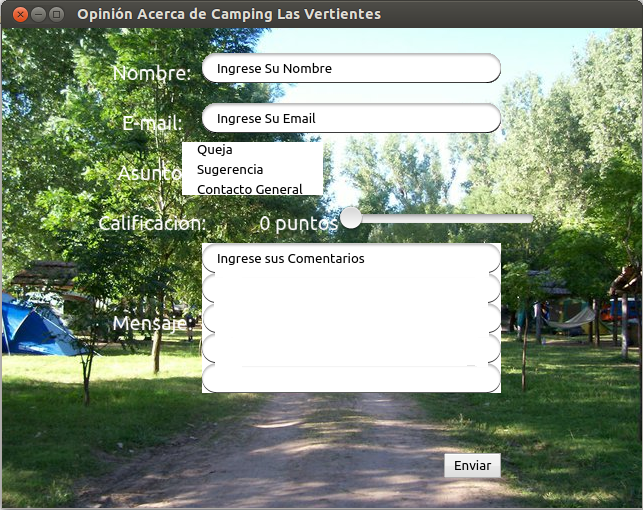
\includegraphics{Opinia.png}

Este ejemplo es el modelo que utiliza a la compañia básica del proyecto, el ``Camping Las Vertientes''.


\section{Descarga}
\label{Opinia:descarga}
La descarga de Opinia, se puede dar desde su repositorio en GitHub, ingresando el siguiente comando en la terminal de linux:


\section{Código Python}
\label{Opinia:codigo-python}

\subsection{Opinia.py}
\label{Opinia:opinia-py}
\begin{notice}{note}{Nota:}
Se debe editar el archivo de configuración presente en ''.Data/conf.ini''
\end{notice}

\begin{Verbatim}[commandchars=\\\{\},numbers=left,firstnumber=1,stepnumber=1]
\PYG{c}{\PYGZsh{}!/usr/bin/env python}
\PYG{c}{\PYGZsh{} -*- coding: utf-8 -*-}

\PYG{l+s+sd}{"""Importamos los modulos"""}
\PYG{k+kn}{import} \PYG{n+nn}{pilas}
\PYG{k+kn}{import} \PYG{n+nn}{sys}
\PYG{k+kn}{import} \PYG{n+nn}{Multilinea}
\PYG{k+kn}{import} \PYG{n+nn}{ConfigParser}
\PYG{k+kn}{import} \PYG{n+nn}{urllib}

\PYG{l+s+sd}{"""Creamos y Configuramos todas las funciones"""}

\PYG{k}{def} \PYG{n+nf}{cuando\PYGZus{}hacen\PYGZus{}click}\PYG{p}{(}\PYG{p}{)}\PYG{p}{:}
    \PYG{l+s+sd}{"""Esta funcion es el evento que actuara cuando se haga click en el boton "Enviar" """}


    \PYG{l+s+sd}{"""Capturamos y Guardamos los datos del Formulario"""}
    \PYG{n}{pilas}\PYG{o}{.}\PYG{n}{avisar}\PYG{p}{(}\PYG{l+s}{"}\PYG{l+s}{Aguarde por favor, el formulario esta siendo enviado}\PYG{l+s}{"}\PYG{p}{)}
    \PYG{n}{cfgFile\PYGZus{}w} \PYG{o}{=} \PYG{n+nb}{open}\PYG{p}{(}\PYG{l+s}{"}\PYG{l+s}{.Data/datos.ini}\PYG{l+s}{"}\PYG{p}{,}\PYG{l+s}{'}\PYG{l+s}{w}\PYG{l+s}{'}\PYG{p}{)}
    \PYG{n}{C}\PYG{o}{.}\PYG{n}{set}\PYG{p}{(}\PYG{l+s}{'}\PYG{l+s}{datos}\PYG{l+s}{'}\PYG{p}{,}\PYG{l+s}{'}\PYG{l+s}{nombre}\PYG{l+s}{'}\PYG{p}{,} \PYG{n}{txtNombre}\PYG{o}{.}\PYG{n}{texto}\PYG{p}{)}
    \PYG{n}{C}\PYG{o}{.}\PYG{n}{write}\PYG{p}{(}\PYG{n}{cfgFile\PYGZus{}w}\PYG{p}{)}
    \PYG{n}{C}\PYG{o}{.}\PYG{n}{set}\PYG{p}{(}\PYG{l+s}{'}\PYG{l+s}{datos}\PYG{l+s}{'}\PYG{p}{,}\PYG{l+s}{'}\PYG{l+s}{email}\PYG{l+s}{'}\PYG{p}{,} \PYG{n}{txtEmail}\PYG{o}{.}\PYG{n}{texto}\PYG{p}{)}
    \PYG{n}{C}\PYG{o}{.}\PYG{n}{write}\PYG{p}{(}\PYG{n}{cfgFile\PYGZus{}w}\PYG{p}{)}
    \PYG{n}{cfgFile\PYGZus{}w}\PYG{o}{.}\PYG{n}{close}\PYG{p}{(}\PYG{p}{)}
    \PYG{n}{guardarmensaje} \PYG{o}{=} \PYG{n+nb}{open}\PYG{p}{(}\PYG{l+s}{"}\PYG{l+s}{.Data/mensaje.txt}\PYG{l+s}{"}\PYG{p}{,}\PYG{l+s}{"}\PYG{l+s}{w}\PYG{l+s}{"}\PYG{p}{)}
    \PYG{n}{guardarmensaje}\PYG{o}{.}\PYG{n}{write}\PYG{p}{(}\PYG{n}{txtMensaje}\PYG{o}{.}\PYG{n}{texto}\PYG{p}{)}
    \PYG{n}{guardarmensaje}\PYG{o}{.}\PYG{n}{close}\PYG{p}{(}\PYG{p}{)}

    \PYG{l+s+sd}{"""Disparamos las funciones que enviara el email y otra que creara el archivo html, para luego ser subido por otra funcion"""}
    \PYG{n}{enviar\PYGZus{}email}\PYG{p}{(}\PYG{p}{)}
    \PYG{n}{bajar\PYGZus{}html}\PYG{p}{(}\PYG{p}{)}

    \PYG{l+s+sd}{"""Ahora se limpiaran los campos y se reiniciara el formulario"""}
    \PYG{n}{limpiar}\PYG{o}{=}\PYG{n+nb}{open}\PYG{p}{(}\PYG{l+s}{"}\PYG{l+s}{.Data/datos.ini}\PYG{l+s}{"}\PYG{p}{,}\PYG{l+s}{"}\PYG{l+s}{w}\PYG{l+s}{"}\PYG{p}{)}
    \PYG{n}{limpiar}\PYG{o}{.}\PYG{n}{write}\PYG{p}{(}\PYG{l+s}{"}\PYG{l+s}{[datos]}\PYG{l+s+se}{\PYGZbs{}n}\PYG{l+s}{nombre = }\PYG{l+s+se}{\PYGZbs{}n}\PYG{l+s}{email = }\PYG{l+s+se}{\PYGZbs{}n}\PYG{l+s}{asunto = }\PYG{l+s+se}{\PYGZbs{}n}\PYG{l+s}{calificacion = }\PYG{l+s}{"}\PYG{p}{)}
    \PYG{n}{limpiar}\PYG{o}{.}\PYG{n}{close}\PYG{p}{(}\PYG{p}{)}
    \PYG{n}{limpiar2}\PYG{o}{=}\PYG{n+nb}{open}\PYG{p}{(}\PYG{l+s}{"}\PYG{l+s}{.Data/mensaje.txt}\PYG{l+s}{"}\PYG{p}{,}\PYG{l+s}{"}\PYG{l+s}{w}\PYG{l+s}{"}\PYG{p}{)}
    \PYG{n}{limpiar2}\PYG{o}{.}\PYG{n}{write}\PYG{p}{(}\PYG{l+s}{"}\PYG{l+s}{"}\PYG{p}{)}
    \PYG{n}{limpiar2}\PYG{o}{.}\PYG{n}{close}\PYG{p}{(}\PYG{p}{)}
    \PYG{n}{txtNombre}\PYG{o}{.}\PYG{n}{texto} \PYG{o}{=} \PYG{l+s}{"}\PYG{l+s}{Ingrese su Nombre}\PYG{l+s}{"}
    \PYG{n}{txtEmail}\PYG{o}{.}\PYG{n}{texto} \PYG{o}{=} \PYG{l+s}{"}\PYG{l+s}{Ingrese su Email}\PYG{l+s}{"}
    \PYG{n}{txtMensaje}\PYG{o}{.}\PYG{n}{texto} \PYG{o}{=} \PYG{l+s}{u"}\PYG{l+s}{Ingrese sus Comentarios}\PYG{l+s}{"}
    \PYG{n}{cuando\PYGZus{}cambia\PYGZus{}Calificacion}\PYG{p}{(}\PYG{l+m+mi}{0}\PYG{p}{)}

    \PYG{l+s+sd}{"""Si todo ha sido procesado correctamente, notificamos la aceptacion"""}
    \PYG{n}{pilas}\PYG{o}{.}\PYG{n}{avisar}\PYG{p}{(}\PYG{l+s}{u'}\PYG{l+s}{Se envió el formulario}\PYG{l+s}{'}\PYG{p}{)}
    \PYG{k}{print} \PYG{l+s}{u'}\PYG{l+s}{Se envió el formulario Correctamente}\PYG{l+s}{'}


\PYG{k}{def} \PYG{n+nf}{cuando\PYGZus{}selecciona\PYGZus{}Asunto}\PYG{p}{(}\PYG{n}{opcion\PYGZus{}seleccionada}\PYG{p}{)}\PYG{p}{:}
    \PYG{l+s+sd}{"""Esta funcion es el evento que actuara al seleccionar una alternativa del Campo de Opcion"""}
    \PYG{n}{pilas}\PYG{o}{.}\PYG{n}{avisar}\PYG{p}{(}\PYG{l+s}{"}\PYG{l+s}{Ha seleccionado la opcion: }\PYG{l+s}{"} \PYG{o}{+} \PYG{n}{opcion\PYGZus{}seleccionada}\PYG{p}{)}
    \PYG{n}{cfgFile\PYGZus{}w} \PYG{o}{=} \PYG{n+nb}{open}\PYG{p}{(}\PYG{l+s}{"}\PYG{l+s}{.Data/datos.ini}\PYG{l+s}{"}\PYG{p}{,}\PYG{l+s}{'}\PYG{l+s}{w}\PYG{l+s}{'}\PYG{p}{)}
    \PYG{n}{C}\PYG{o}{.}\PYG{n}{set}\PYG{p}{(}\PYG{l+s}{'}\PYG{l+s}{datos}\PYG{l+s}{'}\PYG{p}{,}\PYG{l+s}{'}\PYG{l+s}{asunto}\PYG{l+s}{'}\PYG{p}{,} \PYG{n}{opcion\PYGZus{}seleccionada}\PYG{p}{)}
    \PYG{n}{C}\PYG{o}{.}\PYG{n}{write}\PYG{p}{(}\PYG{n}{cfgFile\PYGZus{}w}\PYG{p}{)}
    \PYG{n}{cfgFile\PYGZus{}w}\PYG{o}{.}\PYG{n}{close}\PYG{p}{(}\PYG{p}{)}
    \PYG{k}{return} \PYG{n+nb+bp}{None}

\PYG{k}{def} \PYG{n+nf}{cuando\PYGZus{}cambia\PYGZus{}Calificacion}\PYG{p}{(}\PYG{n}{valor}\PYG{p}{)}\PYG{p}{:}
    \PYG{l+s+sd}{"""Esta funcion es el evento que actua cuando se cambia el valor del Campo Deslizante """}
    \PYG{n}{lblCalificacionTotal}\PYG{o}{.}\PYG{n}{definir\PYGZus{}texto}\PYG{p}{(}\PYG{n+nb}{str}\PYG{p}{(}\PYG{n+nb}{int}\PYG{p}{(}\PYG{n}{valor} \PYG{o}{*} \PYG{l+m+mi}{10}\PYG{p}{)}\PYG{p}{)} \PYG{o}{+}\PYG{l+s}{u'}\PYG{l+s}{ puntos}\PYG{l+s}{'}\PYG{p}{)}
    \PYG{n}{cfgFile\PYGZus{}w} \PYG{o}{=} \PYG{n+nb}{open}\PYG{p}{(}\PYG{l+s}{"}\PYG{l+s}{.Data/datos.ini}\PYG{l+s}{"}\PYG{p}{,}\PYG{l+s}{'}\PYG{l+s}{w}\PYG{l+s}{'}\PYG{p}{)}
    \PYG{n}{C}\PYG{o}{.}\PYG{n}{set}\PYG{p}{(}\PYG{l+s}{'}\PYG{l+s}{datos}\PYG{l+s}{'}\PYG{p}{,}\PYG{l+s}{'}\PYG{l+s}{calificacion}\PYG{l+s}{'}\PYG{p}{,} \PYG{n+nb}{str}\PYG{p}{(}\PYG{n+nb}{int}\PYG{p}{(}\PYG{n}{valor} \PYG{o}{*} \PYG{l+m+mi}{10}\PYG{p}{)}\PYG{p}{)} \PYG{o}{+}\PYG{l+s}{u'}\PYG{l+s}{ puntos}\PYG{l+s}{'}\PYG{p}{)}
    \PYG{n}{C}\PYG{o}{.}\PYG{n}{write}\PYG{p}{(}\PYG{n}{cfgFile\PYGZus{}w}\PYG{p}{)}
    \PYG{n}{cfgFile\PYGZus{}w}\PYG{o}{.}\PYG{n}{close}\PYG{p}{(}\PYG{p}{)}

\PYG{k}{def} \PYG{n+nf}{bajar\PYGZus{}html}\PYG{p}{(}\PYG{p}{)}\PYG{p}{:}
    \PYG{l+s+sd}{"""Esta funcion es la que descargara el archivo html del sitio web y luego se lo entregara a la fucion que lo preparara para luego subirlo"""}
    \PYG{k}{def} \PYG{n+nf}{reporthook}\PYG{p}{(}\PYG{o}{*}\PYG{n}{a}\PYG{p}{)}\PYG{p}{:} \PYG{k}{print} \PYG{n}{a}

    \PYG{n}{C} \PYG{o}{=} \PYG{n}{ConfigParser}\PYG{o}{.}\PYG{n}{ConfigParser}\PYG{p}{(}\PYG{p}{)}
    \PYG{n}{C}\PYG{o}{.}\PYG{n}{read}\PYG{p}{(}\PYG{l+s}{"}\PYG{l+s}{.Data/conf.ini}\PYG{l+s}{"}\PYG{p}{)}
    \PYG{n}{web} \PYG{o}{=} \PYG{n}{C}\PYG{o}{.}\PYG{n}{get}\PYG{p}{(}\PYG{l+s}{"}\PYG{l+s}{SMTP}\PYG{l+s}{"}\PYG{p}{,}\PYG{l+s}{"}\PYG{l+s}{sitio-web}\PYG{l+s}{"}\PYG{p}{)}
    \PYG{n}{url} \PYG{o}{=} \PYG{n}{web}\PYG{o}{+}\PYG{l+s}{"}\PYG{l+s}{Opiniones/Opiniones.html}\PYG{l+s}{"}
    \PYG{n+nb}{file} \PYG{o}{=} \PYG{l+s}{"}\PYG{l+s}{.Data/Opiniones.html}\PYG{l+s}{"}
    \PYG{n}{urllib}\PYG{o}{.}\PYG{n}{urlretrieve}\PYG{p}{(}\PYG{n}{url}\PYG{p}{,} \PYG{n+nb}{file}\PYG{p}{,} \PYG{n}{reporthook}\PYG{p}{)}
    \PYG{n}{crear\PYGZus{}html}\PYG{p}{(}\PYG{p}{)}

\PYG{k}{def} \PYG{n+nf}{crear\PYGZus{}html}\PYG{p}{(}\PYG{p}{)}\PYG{p}{:}

    \PYG{l+s+sd}{"""Esta es la funcion que creara el informe HTML para luego ser subidos a la web"""}

    \PYG{k+kn}{from} \PYG{n+nn}{ftplib} \PYG{k+kn}{import} \PYG{n}{FTP}
    \PYG{n}{C}\PYG{o}{.}\PYG{n}{read}\PYG{p}{(}\PYG{l+s}{"}\PYG{l+s}{.Data/conf.ini}\PYG{l+s}{"}\PYG{p}{)}
    \PYG{n}{usuario} \PYG{o}{=} \PYG{n}{C}\PYG{o}{.}\PYG{n}{get}\PYG{p}{(}\PYG{l+s}{"}\PYG{l+s}{FTP}\PYG{l+s}{"}\PYG{p}{,}\PYG{l+s}{"}\PYG{l+s}{usuario}\PYG{l+s}{"}\PYG{p}{)}
    \PYG{n}{servidor} \PYG{o}{=} \PYG{n}{C}\PYG{o}{.}\PYG{n}{get}\PYG{p}{(}\PYG{l+s}{"}\PYG{l+s}{FTP}\PYG{l+s}{"}\PYG{p}{,}\PYG{l+s}{"}\PYG{l+s}{servidor}\PYG{l+s}{"}\PYG{p}{)}
    \PYG{n}{password} \PYG{o}{=} \PYG{n}{C}\PYG{o}{.}\PYG{n}{get}\PYG{p}{(}\PYG{l+s}{"}\PYG{l+s}{FTP}\PYG{l+s}{"}\PYG{p}{,}\PYG{l+s}{"}\PYG{l+s}{password}\PYG{l+s}{"}\PYG{p}{)}
    \PYG{n}{ftp} \PYG{o}{=} \PYG{n}{FTP}\PYG{p}{(}\PYG{n}{servidor}\PYG{p}{)}\PYG{p}{;}
    \PYG{n}{ftp}\PYG{o}{.}\PYG{n}{login}\PYG{p}{(}\PYG{n}{user}\PYG{o}{=}\PYG{n}{usuario}\PYG{p}{,} \PYG{n}{passwd}\PYG{o}{=}\PYG{n}{password}\PYG{p}{)}
    \PYG{n}{ftp}\PYG{o}{.}\PYG{n}{cwd}\PYG{p}{(}\PYG{l+s}{"}\PYG{l+s}{/public\PYGZus{}html/Opiniones/}\PYG{l+s}{"}\PYG{p}{)}\PYG{p}{;}
    \PYG{n}{ftp}\PYG{o}{.}\PYG{n}{retrbinary}\PYG{p}{(}\PYG{l+s}{"}\PYG{l+s}{RETR Opiniones.html}\PYG{l+s}{"}\PYG{p}{,}\PYG{n+nb}{open}\PYG{p}{(}\PYG{l+s}{"}\PYG{l+s}{.Data/Opiniones.html}\PYG{l+s}{"}\PYG{p}{,}\PYG{l+s}{"}\PYG{l+s}{wb}\PYG{l+s}{"}\PYG{p}{)}\PYG{o}{.}\PYG{n}{write}\PYG{p}{)}
    \PYG{n}{ftp}\PYG{o}{.}\PYG{n}{quit}\PYG{p}{(}\PYG{p}{)}

    \PYG{l+s+sd}{"""Cargamos los datos para crear el archivo html"""}
    \PYG{n}{C}\PYG{o}{.}\PYG{n}{read}\PYG{p}{(}\PYG{l+s}{"}\PYG{l+s}{.Data/datos.ini}\PYG{l+s}{"}\PYG{p}{)}
    \PYG{n}{nombre} \PYG{o}{=} \PYG{n}{C}\PYG{o}{.}\PYG{n}{get}\PYG{p}{(}\PYG{l+s}{"}\PYG{l+s}{datos}\PYG{l+s}{"}\PYG{p}{,}\PYG{l+s}{'}\PYG{l+s}{nombre}\PYG{l+s}{'}\PYG{p}{)}
    \PYG{n}{email} \PYG{o}{=} \PYG{n}{C}\PYG{o}{.}\PYG{n}{get}\PYG{p}{(}\PYG{l+s}{"}\PYG{l+s}{datos}\PYG{l+s}{"}\PYG{p}{,}\PYG{l+s}{'}\PYG{l+s}{email}\PYG{l+s}{'}\PYG{p}{)}
    \PYG{n}{asunto} \PYG{o}{=} \PYG{n}{C}\PYG{o}{.}\PYG{n}{get}\PYG{p}{(}\PYG{l+s}{"}\PYG{l+s}{datos}\PYG{l+s}{"}\PYG{p}{,}\PYG{l+s}{'}\PYG{l+s}{asunto}\PYG{l+s}{'}\PYG{p}{)}
    \PYG{n}{calificacion} \PYG{o}{=} \PYG{n}{C}\PYG{o}{.}\PYG{n}{get}\PYG{p}{(}\PYG{l+s}{"}\PYG{l+s}{datos}\PYG{l+s}{"}\PYG{p}{,}\PYG{l+s}{'}\PYG{l+s}{calificacion}\PYG{l+s}{'}\PYG{p}{)}
    \PYG{n}{mensaje} \PYG{o}{=} \PYG{n+nb}{open}\PYG{p}{(}\PYG{l+s}{"}\PYG{l+s}{.Data/mensaje.txt}\PYG{l+s}{"}\PYG{p}{,}\PYG{l+s}{'}\PYG{l+s}{r}\PYG{l+s}{'}\PYG{p}{)}
    \PYG{n}{mensajea} \PYG{o}{=} \PYG{n}{mensaje}\PYG{o}{.}\PYG{n}{read}\PYG{p}{(}\PYG{p}{)}
    \PYG{n}{mensaje}\PYG{o}{.}\PYG{n}{close}\PYG{p}{(}\PYG{p}{)}

    \PYG{l+s+sd}{"""Guardamos el archivo html"""}
    \PYG{n}{creararchivo} \PYG{o}{=} \PYG{n+nb}{open}\PYG{p}{(}\PYG{l+s}{"}\PYG{l+s}{.Data/Opiniones.html}\PYG{l+s}{"}\PYG{p}{,}\PYG{l+s}{"}\PYG{l+s}{a}\PYG{l+s}{"}\PYG{p}{)}
    \PYG{n}{creararchivo}\PYG{o}{.}\PYG{n}{write}\PYG{p}{(}\PYG{n+nb}{str}\PYG{p}{(}\PYG{l+s}{"}\PYG{l+s+se}{\PYGZbs{}n}\PYG{l+s}{\PYGZlt{}hr\PYGZgt{}Nombre: }\PYG{l+s}{"}\PYG{o}{+}\PYG{n}{nombre}\PYG{o}{+}\PYG{l+s}{"}\PYG{l+s}{\PYGZlt{}br\PYGZgt{}Email: \PYGZlt{}a href=mailto:}\PYG{l+s}{"}\PYG{o}{+}\PYG{n}{email}\PYG{o}{+}\PYG{l+s}{"}\PYG{l+s}{\PYGZgt{}}\PYG{l+s}{"}\PYG{o}{+}\PYG{n}{email}\PYG{o}{+}\PYG{l+s}{"}\PYG{l+s}{\PYGZlt{}/a\PYGZgt{}\PYGZlt{}br\PYGZgt{}Asunto: }\PYG{l+s}{"}\PYG{o}{+}\PYG{n}{asunto}\PYG{o}{+}\PYG{l+s}{"}\PYG{l+s}{\PYGZlt{}br\PYGZgt{}Calificacion: }\PYG{l+s}{"}\PYG{o}{+}\PYG{n}{calificacion}\PYG{o}{+}\PYG{l+s}{"}\PYG{l+s}{\PYGZlt{}br\PYGZgt{}Comentarios: }\PYG{l+s}{"}\PYG{o}{+}\PYG{n}{mensajea}\PYG{p}{)}\PYG{p}{)}
    \PYG{n}{creararchivo}\PYG{o}{.}\PYG{n}{close}\PYG{p}{(}\PYG{p}{)}

    \PYG{l+s+sd}{"""Disparamos la funcion que subira el archivo html"""}
    \PYG{n}{subir\PYGZus{}html}\PYG{p}{(}\PYG{p}{)}

\PYG{k}{def} \PYG{n+nf}{enviar\PYGZus{}email}\PYG{p}{(}\PYG{p}{)}\PYG{p}{:}
    \PYG{l+s+sd}{"""Esta es la funcion que enviara el email notificando de una nueva opinion"""}

    \PYG{l+s+sd}{"""Importamos la libreria necesaria y cargamos los datos para luego ser enviados"""}
    \PYG{k+kn}{import} \PYG{n+nn}{smtplib}
    \PYG{n}{C} \PYG{o}{=} \PYG{n}{ConfigParser}\PYG{o}{.}\PYG{n}{ConfigParser}\PYG{p}{(}\PYG{p}{)}
    \PYG{n}{C}\PYG{o}{.}\PYG{n}{read}\PYG{p}{(}\PYG{l+s}{"}\PYG{l+s}{.Data/datos.ini}\PYG{l+s}{"}\PYG{p}{)}
    \PYG{n}{nombre} \PYG{o}{=} \PYG{n}{C}\PYG{o}{.}\PYG{n}{get}\PYG{p}{(}\PYG{l+s}{"}\PYG{l+s}{datos}\PYG{l+s}{"}\PYG{p}{,}\PYG{l+s}{"}\PYG{l+s}{nombre}\PYG{l+s}{"}\PYG{p}{)}
    \PYG{n}{email} \PYG{o}{=} \PYG{n}{C}\PYG{o}{.}\PYG{n}{get}\PYG{p}{(}\PYG{l+s}{"}\PYG{l+s}{datos}\PYG{l+s}{"}\PYG{p}{,}\PYG{l+s}{"}\PYG{l+s}{email}\PYG{l+s}{"}\PYG{p}{)}
    \PYG{n}{asunto} \PYG{o}{=} \PYG{n}{C}\PYG{o}{.}\PYG{n}{get}\PYG{p}{(}\PYG{l+s}{"}\PYG{l+s}{datos}\PYG{l+s}{"}\PYG{p}{,}\PYG{l+s}{"}\PYG{l+s}{asunto}\PYG{l+s}{"}\PYG{p}{)}
    \PYG{n}{calificacion} \PYG{o}{=} \PYG{n}{C}\PYG{o}{.}\PYG{n}{get}\PYG{p}{(}\PYG{l+s}{"}\PYG{l+s}{datos}\PYG{l+s}{"}\PYG{p}{,}\PYG{l+s}{"}\PYG{l+s}{calificacion}\PYG{l+s}{"}\PYG{p}{)}
    \PYG{n}{cargarmensaje} \PYG{o}{=} \PYG{n+nb}{open}\PYG{p}{(}\PYG{l+s}{"}\PYG{l+s}{.Data/mensaje.txt}\PYG{l+s}{"}\PYG{p}{,}\PYG{l+s}{"}\PYG{l+s}{r}\PYG{l+s}{"}\PYG{p}{)}
    \PYG{n}{mensaje}\PYG{o}{=}\PYG{n}{cargarmensaje}\PYG{o}{.}\PYG{n}{read}\PYG{p}{(}\PYG{p}{)}
    \PYG{n}{cargarmensaje}\PYG{o}{.}\PYG{n}{close}\PYG{p}{(}\PYG{p}{)}
    \PYG{n}{C}\PYG{o}{.}\PYG{n}{read}\PYG{p}{(}\PYG{l+s}{"}\PYG{l+s}{.Data/conf.ini}\PYG{l+s}{"}\PYG{p}{)}
    \PYG{n}{web} \PYG{o}{=} \PYG{n}{C}\PYG{o}{.}\PYG{n}{get}\PYG{p}{(}\PYG{l+s}{"}\PYG{l+s}{SMTP}\PYG{l+s}{"}\PYG{p}{,}\PYG{l+s}{"}\PYG{l+s}{sitio-web}\PYG{l+s}{"}\PYG{p}{)}
    \PYG{n}{email2} \PYG{o}{=} \PYG{n}{C}\PYG{o}{.}\PYG{n}{get}\PYG{p}{(}\PYG{l+s}{"}\PYG{l+s}{SMTP}\PYG{l+s}{"}\PYG{p}{,}\PYG{l+s}{"}\PYG{l+s}{email}\PYG{l+s}{"}\PYG{p}{)}
    \PYG{n}{clave} \PYG{o}{=} \PYG{n}{C}\PYG{o}{.}\PYG{n}{get}\PYG{p}{(}\PYG{l+s}{"}\PYG{l+s}{SMTP}\PYG{l+s}{"}\PYG{p}{,}\PYG{l+s}{"}\PYG{l+s}{password}\PYG{l+s}{"}\PYG{p}{)}

    \PYG{l+s+sd}{"""Importamos los modulos adicionales necesarios"""}
    \PYG{k+kn}{from} \PYG{n+nn}{email.mime.text} \PYG{k+kn}{import} \PYG{n}{MIMEText}

    \PYG{l+s+sd}{"""Creamos el mensaje"""}
    \PYG{n}{cuerpodelmensaje} \PYG{o}{=} \PYG{n+nb}{str}\PYG{p}{(}\PYG{l+s}{"}\PYG{l+s}{Nombre: }\PYG{l+s}{"}\PYG{o}{+}\PYG{n}{nombre}\PYG{o}{+}\PYG{l+s}{"}\PYG{l+s+se}{\PYGZbs{}n}\PYG{l+s}{"}\PYG{o}{+}\PYG{l+s}{"}\PYG{l+s}{E-mail: }\PYG{l+s}{"}\PYG{o}{+}\PYG{n}{email}\PYG{o}{+}\PYG{l+s}{"}\PYG{l+s+se}{\PYGZbs{}n}\PYG{l+s}{"}\PYG{o}{+}\PYG{l+s}{"}\PYG{l+s}{Calificacion: }\PYG{l+s}{"}\PYG{o}{+}\PYG{n}{calificacion}\PYG{o}{+}\PYG{l+s}{"}\PYG{l+s+se}{\PYGZbs{}n}\PYG{l+s}{"}\PYG{o}{+}\PYG{l+s}{"}\PYG{l+s}{Comentarios: }\PYG{l+s}{"}\PYG{o}{+}\PYG{n}{mensaje}\PYG{o}{+}\PYG{l+s}{"}\PYG{l+s+se}{\PYGZbs{}n}\PYG{l+s+se}{\PYGZbs{}n}\PYG{l+s}{Ver todos las Opiniones Recibidas}\PYG{l+s+se}{\PYGZbs{}n}\PYG{l+s}{"}\PYG{o}{+}\PYG{n}{web}\PYG{o}{+}\PYG{l+s}{"}\PYG{l+s}{Opiniones/Opiniones.html}\PYG{l+s}{"}\PYG{p}{)}
    \PYG{n}{msg} \PYG{o}{=} \PYG{n}{MIMEText}\PYG{p}{(}\PYG{n}{cuerpodelmensaje}\PYG{p}{)}

    \PYG{l+s+sd}{"""Conectamos con el server"""}
    \PYG{n}{msg}\PYG{p}{[}\PYG{l+s}{'}\PYG{l+s}{Subject}\PYG{l+s}{'}\PYG{p}{]} \PYG{o}{=} \PYG{l+s}{'}\PYG{l+s}{Usted ha recibido una nueva opinion - }\PYG{l+s}{'}\PYG{o}{+}\PYG{n}{asunto}
    \PYG{n}{msg}\PYG{p}{[}\PYG{l+s}{'}\PYG{l+s}{From}\PYG{l+s}{'}\PYG{p}{]} \PYG{o}{=} \PYG{n}{email}
    \PYG{n}{msg}\PYG{p}{[}\PYG{l+s}{'}\PYG{l+s}{To}\PYG{l+s}{'}\PYG{p}{]} \PYG{o}{=} \PYG{n}{email2}

    \PYG{l+s+sd}{"""Autenticamos"""}
    \PYG{n}{mailServer} \PYG{o}{=} \PYG{n}{smtplib}\PYG{o}{.}\PYG{n}{SMTP}\PYG{p}{(}\PYG{l+s}{'}\PYG{l+s}{smtp.gmail.com}\PYG{l+s}{'}\PYG{p}{,}\PYG{l+m+mi}{587}\PYG{p}{)}
    \PYG{n}{mailServer}\PYG{o}{.}\PYG{n}{ehlo}\PYG{p}{(}\PYG{p}{)}
    \PYG{n}{mailServer}\PYG{o}{.}\PYG{n}{starttls}\PYG{p}{(}\PYG{p}{)}
    \PYG{n}{mailServer}\PYG{o}{.}\PYG{n}{ehlo}\PYG{p}{(}\PYG{p}{)}
    \PYG{n}{mailServer}\PYG{o}{.}\PYG{n}{login}\PYG{p}{(}\PYG{n}{email2}\PYG{p}{,} \PYG{n}{clave}\PYG{p}{)}

    \PYG{l+s+sd}{"""Enviamos"""}
    \PYG{n}{mailServer}\PYG{o}{.}\PYG{n}{sendmail}\PYG{p}{(}\PYG{n}{email2}\PYG{p}{,} \PYG{n}{email2}\PYG{p}{,} \PYG{n}{msg}\PYG{o}{.}\PYG{n}{as\PYGZus{}string}\PYG{p}{(}\PYG{p}{)}\PYG{p}{)}

    \PYG{l+s+sd}{"""Cerramos conexion"""}
    \PYG{n}{mailServer}\PYG{o}{.}\PYG{n}{close}\PYG{p}{(}\PYG{p}{)}

\PYG{k}{def} \PYG{n+nf}{subir\PYGZus{}html}\PYG{p}{(}\PYG{p}{)}\PYG{p}{:}
    \PYG{l+s+sd}{"""Esta es la funcion que subira el archivo html al servidor web"""}

    \PYG{l+s+sd}{"""Importamos las librerias necesarias"""}
    \PYG{k+kn}{import} \PYG{n+nn}{ftplib}
    \PYG{k+kn}{import} \PYG{n+nn}{os}

    \PYG{n}{C}\PYG{o}{.}\PYG{n}{read}\PYG{p}{(}\PYG{l+s}{"}\PYG{l+s}{.Data/conf.ini}\PYG{l+s}{"}\PYG{p}{)}
    \PYG{l+s+sd}{""" Cargamos Datos FTP"""}
    \PYG{n}{ftp\PYGZus{}servidor} \PYG{o}{=} \PYG{n}{C}\PYG{o}{.}\PYG{n}{get}\PYG{p}{(}\PYG{l+s}{"}\PYG{l+s}{FTP}\PYG{l+s}{"}\PYG{p}{,}\PYG{l+s}{"}\PYG{l+s}{servidor}\PYG{l+s}{"}\PYG{p}{)}
    \PYG{n}{ftp\PYGZus{}usuario}  \PYG{o}{=} \PYG{n}{C}\PYG{o}{.}\PYG{n}{get}\PYG{p}{(}\PYG{l+s}{"}\PYG{l+s}{FTP}\PYG{l+s}{"}\PYG{p}{,}\PYG{l+s}{"}\PYG{l+s}{usuario}\PYG{l+s}{"}\PYG{p}{)}
    \PYG{n}{ftp\PYGZus{}clave}    \PYG{o}{=} \PYG{n}{C}\PYG{o}{.}\PYG{n}{get}\PYG{p}{(}\PYG{l+s}{"}\PYG{l+s}{FTP}\PYG{l+s}{"}\PYG{p}{,}\PYG{l+s}{"}\PYG{l+s}{password}\PYG{l+s}{"}\PYG{p}{)}
    \PYG{n}{ftp\PYGZus{}raiz}     \PYG{o}{=} \PYG{l+s}{'}\PYG{l+s}{/public\PYGZus{}html/Opiniones/}\PYG{l+s}{'}

    \PYG{l+s+sd}{""" Cargamos Datos del fichero a subir"""}
    \PYG{n}{fichero\PYGZus{}origen} \PYG{o}{=} \PYG{l+s}{'}\PYG{l+s}{.Data/Opiniones.html}\PYG{l+s}{'}
    \PYG{n}{fichero\PYGZus{}destino} \PYG{o}{=} \PYG{l+s}{'}\PYG{l+s}{Opiniones.html}\PYG{l+s}{'}

    \PYG{l+s+sd}{"""Conectamos con el servidor"""}
    \PYG{k}{try}\PYG{p}{:}
            \PYG{n}{s} \PYG{o}{=} \PYG{n}{ftplib}\PYG{o}{.}\PYG{n}{FTP}\PYG{p}{(}\PYG{n}{ftp\PYGZus{}servidor}\PYG{p}{,} \PYG{n}{ftp\PYGZus{}usuario}\PYG{p}{,} \PYG{n}{ftp\PYGZus{}clave}\PYG{p}{)}
            \PYG{k}{try}\PYG{p}{:}
                    \PYG{n}{f} \PYG{o}{=} \PYG{n+nb}{open}\PYG{p}{(}\PYG{n}{fichero\PYGZus{}origen}\PYG{p}{,} \PYG{l+s}{'}\PYG{l+s}{r}\PYG{l+s}{'}\PYG{p}{)}
                    \PYG{n}{s}\PYG{o}{.}\PYG{n}{cwd}\PYG{p}{(}\PYG{n}{ftp\PYGZus{}raiz}\PYG{p}{)}
                    \PYG{n}{s}\PYG{o}{.}\PYG{n}{storbinary}\PYG{p}{(}\PYG{l+s}{'}\PYG{l+s}{STOR }\PYG{l+s}{'} \PYG{o}{+} \PYG{n}{fichero\PYGZus{}destino}\PYG{p}{,} \PYG{n}{f}\PYG{p}{)}
                    \PYG{n}{f}\PYG{o}{.}\PYG{n}{close}\PYG{p}{(}\PYG{p}{)}
                    \PYG{n}{s}\PYG{o}{.}\PYG{n}{quit}\PYG{p}{(}\PYG{p}{)}
            \PYG{k}{except}\PYG{p}{:}
                    \PYG{k}{print} \PYG{l+s}{"}\PYG{l+s}{No se ha podido encontrar el fichero }\PYG{l+s}{"} \PYG{o}{+} \PYG{n}{fichero\PYGZus{}origen}
    \PYG{k}{except}\PYG{p}{:}
            \PYG{k}{print} \PYG{l+s}{"}\PYG{l+s}{No se ha podido conectar al servidor }\PYG{l+s}{"} \PYG{o}{+} \PYG{n}{ftp\PYGZus{}servidor}


\PYG{l+s+sd}{"""Creamos la estructura basica del software"""}

\PYG{l+s+sd}{"""Inicializamos ConfigParser"""}
\PYG{n}{C} \PYG{o}{=} \PYG{n}{ConfigParser}\PYG{o}{.}\PYG{n}{ConfigParser}\PYG{p}{(}\PYG{p}{)}
\PYG{n}{C}\PYG{o}{.}\PYG{n}{read}\PYG{p}{(}\PYG{l+s}{"}\PYG{l+s}{.Data/datos.ini}\PYG{l+s}{"}\PYG{p}{)}

\PYG{l+s+sd}{"""Iniciamos Pilas"""}
\PYG{n}{pilas}\PYG{o}{.}\PYG{n}{iniciar}\PYG{p}{(}\PYG{n}{titulo}\PYG{o}{=}\PYG{l+s}{u"}\PYG{l+s}{Opinión Acerca de Camping Las Vertientes - Opinia}\PYG{l+s}{"}\PYG{p}{)}
\PYG{n}{fondo} \PYG{o}{=} \PYG{n}{pilas}\PYG{o}{.}\PYG{n}{fondos}\PYG{o}{.}\PYG{n}{Fondo}\PYG{p}{(}\PYG{l+s}{"}\PYG{l+s}{.Data/Camping.jpg}\PYG{l+s}{"}\PYG{p}{)}
\PYG{n}{fondo}\PYG{o}{.}\PYG{n}{escala} \PYG{o}{=} \PYG{l+m+mi}{1}
\PYG{n}{posicionV} \PYG{o}{=} \PYG{l+m+mi}{10}
\PYG{n}{posicionL} \PYG{o}{=} \PYG{o}{-}\PYG{l+m+mi}{170}
\PYG{n}{posicionR} \PYG{o}{=} \PYG{l+m+mi}{30}
\PYG{n}{lblEscala} \PYG{o}{=} \PYG{l+m+mf}{0.75}
\PYG{n}{escapar} \PYG{o}{=} \PYG{l+m+mi}{500}
\PYG{n}{Multilinea}\PYG{o}{.}\PYG{n}{inicializar}\PYG{p}{(}\PYG{p}{)}

\PYG{l+s+sd}{""" Creamos el Boton"""}
\PYG{n}{boton} \PYG{o}{=} \PYG{n}{pilas}\PYG{o}{.}\PYG{n}{interfaz}\PYG{o}{.}\PYG{n}{Boton}\PYG{p}{(}\PYG{l+s}{"}\PYG{l+s}{Enviar}\PYG{l+s}{"}\PYG{p}{)}
\PYG{n}{boton}\PYG{o}{.}\PYG{n}{x}\PYG{p}{,}\PYG{n}{boton}\PYG{o}{.}\PYG{n}{y} \PYG{o}{=} \PYG{l+m+mi}{150}\PYG{p}{,}\PYG{o}{-}\PYG{l+m+mi}{200}

\PYG{l+s+sd}{"""Convocamos el evento que actuara cuando se haga click en el boton"""}
\PYG{n}{boton}\PYG{o}{.}\PYG{n}{conectar}\PYG{p}{(}\PYG{n}{cuando\PYGZus{}hacen\PYGZus{}click}\PYG{p}{)}

\PYG{l+s+sd}{"""Creamos y Configuramos Las Entradas de Texto"""}
\PYG{n}{lblNombre} \PYG{o}{=} \PYG{n}{pilas}\PYG{o}{.}\PYG{n}{actores}\PYG{o}{.}\PYG{n}{Texto}\PYG{p}{(}\PYG{l+s}{"}\PYG{l+s}{Nombre:}\PYG{l+s}{"}\PYG{p}{)}
\PYG{n}{lblNombre}\PYG{o}{.}\PYG{n}{escala} \PYG{o}{=} \PYG{n}{lblEscala}
\PYG{n}{lblNombre}\PYG{o}{.}\PYG{n}{x}\PYG{p}{,}\PYG{n}{lblNombre}\PYG{o}{.}\PYG{n}{y} \PYG{o}{=} \PYG{n}{posicionL}\PYG{p}{,}\PYG{p}{(}\PYG{n}{posicionV} \PYG{o}{*}\PYG{l+m+mi}{20}\PYG{p}{)}
\PYG{n}{txtNombre} \PYG{o}{=} \PYG{n}{pilas}\PYG{o}{.}\PYG{n}{interfaz}\PYG{o}{.}\PYG{n}{IngresoDeTexto}\PYG{p}{(}\PYG{n}{limite\PYGZus{}de\PYGZus{}caracteres}\PYG{o}{=}\PYG{l+m+mi}{39}\PYG{p}{,} \PYG{n}{texto\PYGZus{}inicial}\PYG{o}{=}\PYG{l+s}{"}\PYG{l+s}{Ingrese Su Nombre}\PYG{l+s}{"}\PYG{p}{)}
\PYG{n}{txtNombre}\PYG{o}{.}\PYG{n}{x}\PYG{p}{,}\PYG{n}{txtNombre}\PYG{o}{.}\PYG{n}{y} \PYG{o}{=} \PYG{n}{posicionR}\PYG{p}{,}\PYG{p}{(}\PYG{n}{posicionV} \PYG{o}{*}\PYG{l+m+mi}{20}\PYG{p}{)}
\PYG{n}{lblEmail} \PYG{o}{=} \PYG{n}{pilas}\PYG{o}{.}\PYG{n}{actores}\PYG{o}{.}\PYG{n}{Texto}\PYG{p}{(}\PYG{l+s}{"}\PYG{l+s}{E-mail:}\PYG{l+s}{"}\PYG{p}{)}
\PYG{n}{lblEmail}\PYG{o}{.}\PYG{n}{escala} \PYG{o}{=} \PYG{n}{lblEscala}
\PYG{n}{lblEmail}\PYG{o}{.}\PYG{n}{x}\PYG{p}{,}\PYG{n}{lblEmail}\PYG{o}{.}\PYG{n}{y} \PYG{o}{=} \PYG{n}{posicionL}\PYG{p}{,}\PYG{p}{(}\PYG{n}{posicionV} \PYG{o}{*}\PYG{l+m+mi}{15}\PYG{p}{)}
\PYG{n}{txtEmail} \PYG{o}{=} \PYG{n}{pilas}\PYG{o}{.}\PYG{n}{interfaz}\PYG{o}{.}\PYG{n}{IngresoDeTexto}\PYG{p}{(}\PYG{n}{limite\PYGZus{}de\PYGZus{}caracteres}\PYG{o}{=}\PYG{l+m+mi}{39}\PYG{p}{,} \PYG{n}{texto\PYGZus{}inicial}\PYG{o}{=}\PYG{l+s}{"}\PYG{l+s}{Ingrese Su Email}\PYG{l+s}{"}\PYG{p}{)}
\PYG{n}{txtEmail}\PYG{o}{.}\PYG{n}{x}\PYG{p}{,}\PYG{n}{txtEmail}\PYG{o}{.}\PYG{n}{y} \PYG{o}{=} \PYG{n}{posicionR}\PYG{p}{,}\PYG{p}{(}\PYG{n}{posicionV} \PYG{o}{*}\PYG{l+m+mi}{15}\PYG{p}{)}

\PYG{l+s+sd}{"""Creamos y Configuramos el Campo de Opcion"""}
\PYG{n}{lblAsunto} \PYG{o}{=} \PYG{n}{pilas}\PYG{o}{.}\PYG{n}{actores}\PYG{o}{.}\PYG{n}{Texto}\PYG{p}{(}\PYG{l+s}{"}\PYG{l+s}{Asunto:}\PYG{l+s}{"}\PYG{p}{)}
\PYG{n}{lblAsunto}\PYG{o}{.}\PYG{n}{escala} \PYG{o}{=} \PYG{n}{lblEscala}
\PYG{n}{lblAsunto}\PYG{o}{.}\PYG{n}{x}\PYG{p}{,}\PYG{n}{lblAsunto}\PYG{o}{.}\PYG{n}{y} \PYG{o}{=} \PYG{n}{posicionL}\PYG{p}{,}\PYG{p}{(}\PYG{n}{posicionV} \PYG{o}{*}\PYG{l+m+mi}{10}\PYG{p}{)}
\PYG{n}{opcionesAsunto} \PYG{o}{=} \PYG{n}{pilas}\PYG{o}{.}\PYG{n}{interfaz}\PYG{o}{.}\PYG{n}{ListaSeleccion}\PYG{p}{(}\PYG{p}{[}\PYG{l+s}{'}\PYG{l+s}{Queja}\PYG{l+s}{'}\PYG{p}{,} \PYG{l+s}{'}\PYG{l+s}{Sugerencia}\PYG{l+s}{'}\PYG{p}{,}\PYG{l+s}{'}\PYG{l+s}{Contacto General}\PYG{l+s}{'}\PYG{p}{]}\PYG{p}{,} \PYG{n}{cuando\PYGZus{}selecciona\PYGZus{}Asunto}\PYG{p}{)}
\PYG{n}{opcionesAsunto}\PYG{o}{.}\PYG{n}{x}\PYG{p}{,}\PYG{n}{opcionesAsunto}\PYG{o}{.}\PYG{n}{y} \PYG{o}{=} \PYG{n}{posicionR}\PYG{o}{-}\PYG{l+m+mi}{100}\PYG{p}{,}\PYG{p}{(}\PYG{n}{posicionV} \PYG{o}{*}\PYG{l+m+mi}{10}\PYG{p}{)}

\PYG{l+s+sd}{"""Creamos el campo Mensaje"""}
\PYG{n}{lblMensaje} \PYG{o}{=} \PYG{n}{pilas}\PYG{o}{.}\PYG{n}{actores}\PYG{o}{.}\PYG{n}{Texto}\PYG{p}{(}\PYG{l+s}{"}\PYG{l+s}{Mensaje:}\PYG{l+s}{"}\PYG{p}{)}
\PYG{n}{lblMensaje}\PYG{o}{.}\PYG{n}{escala} \PYG{o}{=} \PYG{n}{lblEscala}
\PYG{n}{lblMensaje}\PYG{o}{.}\PYG{n}{x}\PYG{p}{,}\PYG{n}{lblMensaje}\PYG{o}{.}\PYG{n}{y} \PYG{o}{=} \PYG{n}{posicionL}\PYG{p}{,}\PYG{p}{(}\PYG{n}{posicionV} \PYG{o}{*}\PYG{o}{-}\PYG{l+m+mi}{5}\PYG{p}{)}
\PYG{n}{txtMensaje} \PYG{o}{=} \PYG{n}{Multilinea}\PYG{o}{.}\PYG{n}{EntradaDeTexto}\PYG{p}{(}\PYG{n}{limite\PYGZus{}de\PYGZus{}caracteres}\PYG{o}{=}\PYG{l+m+mi}{235}\PYG{p}{,} \PYG{n}{texto\PYGZus{}inicial}\PYG{o}{=}\PYG{l+s}{u"}\PYG{l+s}{Ingrese sus Comentarios}\PYG{l+s}{"}\PYG{p}{)}
\PYG{n}{txtMensaje}\PYG{o}{.}\PYG{n}{x}\PYG{p}{,}\PYG{n}{txtMensaje}\PYG{o}{.}\PYG{n}{y} \PYG{o}{=} \PYG{n}{posicionR}\PYG{p}{,}\PYG{p}{(}\PYG{n}{posicionV} \PYG{o}{*}\PYG{o}{-}\PYG{l+m+mi}{5}\PYG{p}{)}

\PYG{l+s+sd}{"""Creamos y configuramos el Campo deslizante"""}
\PYG{n}{lblCalificacion} \PYG{o}{=} \PYG{n}{pilas}\PYG{o}{.}\PYG{n}{actores}\PYG{o}{.}\PYG{n}{Texto}\PYG{p}{(}\PYG{l+s}{u"}\PYG{l+s}{Calificación:}\PYG{l+s}{"}\PYG{p}{)}
\PYG{n}{lblCalificacion}\PYG{o}{.}\PYG{n}{escala} \PYG{o}{=} \PYG{n}{lblEscala}
\PYG{n}{lblCalificacion}\PYG{o}{.}\PYG{n}{x}\PYG{p}{,}\PYG{n}{lblCalificacion}\PYG{o}{.}\PYG{n}{y} \PYG{o}{=} \PYG{n}{posicionL}\PYG{p}{,}\PYG{p}{(}\PYG{n}{posicionV} \PYG{o}{*} \PYG{l+m+mi}{5}\PYG{p}{)}
\PYG{n}{lblCalificacionTotal} \PYG{o}{=} \PYG{n}{pilas}\PYG{o}{.}\PYG{n}{actores}\PYG{o}{.}\PYG{n}{Texto}\PYG{p}{(}\PYG{l+s}{u'}\PYG{l+s}{0 puntos}\PYG{l+s}{'}\PYG{p}{)}
\PYG{n}{lblCalificacionTotal}\PYG{o}{.}\PYG{n}{escala} \PYG{o}{=} \PYG{n}{lblEscala}
\PYG{n}{lblCalificacionTotal}\PYG{o}{.}\PYG{n}{x}\PYG{p}{,}\PYG{n}{lblCalificacionTotal}\PYG{o}{.}\PYG{n}{y} \PYG{o}{=} \PYG{n}{posicionL} \PYG{o}{+} \PYG{l+m+mi}{2} \PYG{o}{+} \PYG{n}{lblCalificacion}\PYG{o}{.}\PYG{n}{ancho}\PYG{p}{,}\PYG{p}{(}\PYG{n}{posicionV} \PYG{o}{*} \PYG{l+m+mi}{5}\PYG{p}{)}
\PYG{n}{Calificacion} \PYG{o}{=} \PYG{n}{pilas}\PYG{o}{.}\PYG{n}{interfaz}\PYG{o}{.}\PYG{n}{Deslizador}\PYG{p}{(}\PYG{p}{)}
\PYG{n}{Calificacion}\PYG{o}{.}\PYG{n}{conectar}\PYG{p}{(}\PYG{n}{cuando\PYGZus{}cambia\PYGZus{}Calificacion}\PYG{p}{)}
\PYG{n}{Calificacion}\PYG{o}{.}\PYG{n}{x}\PYG{p}{,}\PYG{n}{Calificacion}\PYG{o}{.}\PYG{n}{y} \PYG{o}{=} \PYG{n}{posicionR}\PYG{p}{,}\PYG{n}{posicionV}\PYG{o}{*}\PYG{l+m+mi}{5}

\PYG{l+s+sd}{"""Ejecutamos el Programa"""}
\PYG{n}{pilas}\PYG{o}{.}\PYG{n}{ejecutar}\PYG{p}{(}\PYG{p}{)}
\end{Verbatim}


\subsection{Multilinea.py}
\label{Opinia:multilinea-py}
\begin{notice}{note}{Nota:}
Este codigo es adicional, ya que Pilas no cuenta con la función Multilinea para una entrada de texto, por lo tanto el código fuente básico provisto por Pilas, ha sido editado por el equipo de ``Opinia'' y su código es el siguiente.
\end{notice}

\begin{Verbatim}[commandchars=\\\{\},numbers=left,firstnumber=1,stepnumber=1]
\PYG{c}{\PYGZsh{} -*- encoding: utf-8 -*-}

\PYG{k+kn}{import} \PYG{n+nn}{pilas}
\PYG{k+kn}{import} \PYG{n+nn}{re}
\PYG{k+kn}{from} \PYG{n+nn}{pilas.interfaz.base\PYGZus{}interfaz} \PYG{k+kn}{import} \PYG{n}{BaseInterfaz}

\PYG{k}{class} \PYG{n+nc}{EntradaDeTexto}\PYG{p}{(}\PYG{n}{BaseInterfaz}\PYG{p}{)}\PYG{p}{:}

    \PYG{k}{def} \PYG{n+nf}{\PYGZus{}\PYGZus{}init\PYGZus{}\PYGZus{}}\PYG{p}{(}\PYG{n+nb+bp}{self}\PYG{p}{,} \PYG{n}{texto\PYGZus{}inicial}\PYG{o}{=}\PYG{l+s}{"}\PYG{l+s}{"}\PYG{p}{,} \PYG{n}{x}\PYG{o}{=}\PYG{l+m+mi}{0}\PYG{p}{,} \PYG{n}{y}\PYG{o}{=}\PYG{l+m+mi}{0}\PYG{p}{,} \PYG{n}{ancho}\PYG{o}{=}\PYG{l+m+mi}{300}\PYG{p}{,} \PYG{n}{limite\PYGZus{}de\PYGZus{}caracteres}\PYG{o}{=}\PYG{l+m+mi}{20}\PYG{p}{,} \PYG{n}{icono}\PYG{o}{=}\PYG{n+nb+bp}{None}\PYG{p}{,} \PYG{n}{acepta\PYGZus{}multilinea}\PYG{o}{=}\PYG{n+nb+bp}{True}\PYG{p}{)}\PYG{p}{:}
        \PYG{n}{BaseInterfaz}\PYG{o}{.}\PYG{n}{\PYGZus{}\PYGZus{}init\PYGZus{}\PYGZus{}}\PYG{p}{(}\PYG{n+nb+bp}{self}\PYG{p}{,} \PYG{n}{x}\PYG{o}{=}\PYG{n}{x}\PYG{p}{,} \PYG{n}{y}\PYG{o}{=}\PYG{n}{y}\PYG{p}{)}
        \PYG{n+nb+bp}{self}\PYG{o}{.}\PYG{n}{texto} \PYG{o}{=} \PYG{n}{texto\PYGZus{}inicial}
        \PYG{n+nb+bp}{self}\PYG{o}{.}\PYG{n}{cursor} \PYG{o}{=} \PYG{l+s}{"}\PYG{l+s}{"}
        \PYG{n+nb+bp}{self}\PYG{o}{.}\PYG{n}{\PYGZus{}cargar\PYGZus{}lienzo}\PYG{p}{(}\PYG{n}{ancho}\PYG{p}{)}
        \PYG{n+nb+bp}{self}\PYG{o}{.}\PYG{n}{acepta\PYGZus{}multilinea} \PYG{o}{=} \PYG{n}{acepta\PYGZus{}multilinea}

        \PYG{k}{if} \PYG{n}{icono}\PYG{p}{:}
            \PYG{n+nb+bp}{self}\PYG{o}{.}\PYG{n}{icono} \PYG{o}{=} \PYG{n}{pilas}\PYG{o}{.}\PYG{n}{imagenes}\PYG{o}{.}\PYG{n}{cargar}\PYG{p}{(}\PYG{n}{icono}\PYG{p}{)}
        \PYG{k}{else}\PYG{p}{:}
            \PYG{n+nb+bp}{self}\PYG{o}{.}\PYG{n}{icono} \PYG{o}{=} \PYG{n+nb+bp}{None}

        \PYG{n+nb+bp}{self}\PYG{o}{.}\PYG{n}{imagen\PYGZus{}caja} \PYG{o}{=} \PYG{n}{pilas}\PYG{o}{.}\PYG{n}{imagenes}\PYG{o}{.}\PYG{n}{cargar}\PYG{p}{(}\PYG{l+s}{"}\PYG{l+s}{.Data/mensaje.png}\PYG{l+s}{"}\PYG{p}{)}
        \PYG{n+nb+bp}{self}\PYG{o}{.}\PYG{n}{centro} \PYG{o}{=} \PYG{p}{(}\PYG{l+s}{"}\PYG{l+s}{centro}\PYG{l+s}{"}\PYG{p}{,} \PYG{l+s}{"}\PYG{l+s}{centro}\PYG{l+s}{"}\PYG{p}{)}
        \PYG{n+nb+bp}{self}\PYG{o}{.}\PYG{n}{\PYGZus{}actualizar\PYGZus{}imagen}\PYG{p}{(}\PYG{p}{)}
        \PYG{n+nb+bp}{self}\PYG{o}{.}\PYG{n}{limite\PYGZus{}de\PYGZus{}caracteres} \PYG{o}{=} \PYG{n}{limite\PYGZus{}de\PYGZus{}caracteres}
        \PYG{n+nb+bp}{self}\PYG{o}{.}\PYG{n}{cualquier\PYGZus{}caracter}\PYG{p}{(}\PYG{p}{)}

        \PYG{n}{pilas}\PYG{o}{.}\PYG{n}{eventos}\PYG{o}{.}\PYG{n}{pulsa\PYGZus{}tecla}\PYG{o}{.}\PYG{n}{conectar}\PYG{p}{(}\PYG{n+nb+bp}{self}\PYG{o}{.}\PYG{n}{cuando\PYGZus{}pulsa\PYGZus{}una\PYGZus{}tecla}\PYG{p}{)}
        \PYG{n}{pilas}\PYG{o}{.}\PYG{n}{mundo}\PYG{o}{.}\PYG{n}{agregar\PYGZus{}tarea\PYGZus{}siempre}\PYG{p}{(}\PYG{l+m+mf}{0.40}\PYG{p}{,} \PYG{n+nb+bp}{self}\PYG{o}{.}\PYG{n}{\PYGZus{}actualizar\PYGZus{}cursor}\PYG{p}{)}
        \PYG{n+nb+bp}{self}\PYG{o}{.}\PYG{n}{fijo} \PYG{o}{=} \PYG{n+nb+bp}{True}

    \PYG{k}{def} \PYG{n+nf}{\PYGZus{}actualizar\PYGZus{}cursor}\PYG{p}{(}\PYG{n+nb+bp}{self}\PYG{p}{)}\PYG{p}{:}
        \PYG{k}{if} \PYG{p}{(}\PYG{n+nb+bp}{self}\PYG{o}{.}\PYG{n}{tiene\PYGZus{}el\PYGZus{}foco}\PYG{p}{)}\PYG{p}{:}
            \PYG{k}{if} \PYG{n+nb+bp}{self}\PYG{o}{.}\PYG{n}{cursor} \PYG{o}{==} \PYG{l+s}{"}\PYG{l+s}{"}\PYG{p}{:}
                \PYG{n+nb+bp}{self}\PYG{o}{.}\PYG{n}{cursor} \PYG{o}{=} \PYG{l+s}{"}\PYG{l+s}{\PYGZus{}}\PYG{l+s}{"}
            \PYG{k}{else}\PYG{p}{:}
                \PYG{n+nb+bp}{self}\PYG{o}{.}\PYG{n}{cursor} \PYG{o}{=} \PYG{l+s}{"}\PYG{l+s}{"}
        \PYG{k}{else}\PYG{p}{:}
            \PYG{n+nb+bp}{self}\PYG{o}{.}\PYG{n}{cursor} \PYG{o}{=} \PYG{l+s}{"}\PYG{l+s}{"}

        \PYG{n+nb+bp}{self}\PYG{o}{.}\PYG{n}{\PYGZus{}actualizar\PYGZus{}imagen}\PYG{p}{(}\PYG{p}{)}
        \PYG{k}{return} \PYG{n+nb+bp}{True}

    \PYG{k}{def} \PYG{n+nf}{cualquier\PYGZus{}caracter}\PYG{p}{(}\PYG{n+nb+bp}{self}\PYG{p}{)}\PYG{p}{:}
        \PYG{n+nb+bp}{self}\PYG{o}{.}\PYG{n}{caracteres\PYGZus{}permitidos} \PYG{o}{=} \PYG{n}{re}\PYG{o}{.}\PYG{n}{compile}\PYG{p}{(}\PYG{l+s}{"}\PYG{l+s}{.*}\PYG{l+s}{"}\PYG{p}{)}

    \PYG{k}{def} \PYG{n+nf}{solo\PYGZus{}numeros}\PYG{p}{(}\PYG{n+nb+bp}{self}\PYG{p}{)}\PYG{p}{:}
        \PYG{n+nb+bp}{self}\PYG{o}{.}\PYG{n}{caracteres\PYGZus{}permitidos} \PYG{o}{=} \PYG{n}{re}\PYG{o}{.}\PYG{n}{compile}\PYG{p}{(}\PYG{l+s}{"}\PYG{l+s}{\PYGZbs{}}\PYG{l+s}{d+}\PYG{l+s}{"}\PYG{p}{)}

    \PYG{k}{def} \PYG{n+nf}{solo\PYGZus{}letras}\PYG{p}{(}\PYG{n+nb+bp}{self}\PYG{p}{)}\PYG{p}{:}
        \PYG{n+nb+bp}{self}\PYG{o}{.}\PYG{n}{caracteres\PYGZus{}permitidos} \PYG{o}{=} \PYG{n}{re}\PYG{o}{.}\PYG{n}{compile}\PYG{p}{(}\PYG{l+s}{"}\PYG{l+s}{[a-z]+}\PYG{l+s}{"}\PYG{p}{)}

    \PYG{k}{def} \PYG{n+nf}{cuando\PYGZus{}pulsa\PYGZus{}una\PYGZus{}tecla}\PYG{p}{(}\PYG{n+nb+bp}{self}\PYG{p}{,} \PYG{n}{evento}\PYG{p}{)}\PYG{p}{:}
        \PYG{n}{leermaximo}\PYG{o}{=}\PYG{n+nb}{open}\PYG{p}{(}\PYG{l+s}{"}\PYG{l+s}{.Data/mensaje.txt}\PYG{l+s}{"}\PYG{p}{,}\PYG{l+s}{"}\PYG{l+s}{r}\PYG{l+s}{"}\PYG{p}{)}
        \PYG{n}{numeromaximo}\PYG{o}{=}\PYG{n+nb}{int}\PYG{p}{(}\PYG{n}{leermaximo}\PYG{o}{.}\PYG{n}{read}\PYG{p}{(}\PYG{p}{)}\PYG{p}{)}
        \PYG{n}{leermaximo}\PYG{o}{.}\PYG{n}{close}\PYG{p}{(}\PYG{p}{)}
        \PYG{k}{if} \PYG{p}{(}\PYG{n+nb+bp}{self}\PYG{o}{.}\PYG{n}{tiene\PYGZus{}el\PYGZus{}foco} \PYG{o+ow}{and} \PYG{n+nb+bp}{self}\PYG{o}{.}\PYG{n}{activo}\PYG{p}{)}\PYG{p}{:}
            \PYG{k}{if} \PYG{n}{evento}\PYG{o}{.}\PYG{n}{codigo} \PYG{o}{==} \PYG{l+s}{'}\PYG{l+s+se}{\PYGZbs{}x08}\PYG{l+s}{'} \PYG{o+ow}{or} \PYG{n}{evento}\PYG{o}{.}\PYG{n}{texto} \PYG{o}{==} \PYG{l+s}{'}\PYG{l+s+se}{\PYGZbs{}x08}\PYG{l+s}{'}\PYG{p}{:}
                \PYG{k}{if} \PYG{n}{numeromaximo} \PYG{o}{==} \PYG{l+m+mi}{0}\PYG{p}{:}
                    \PYG{k}{print} \PYG{l+s}{"}\PYG{l+s}{0}\PYG{l+s}{"}
                \PYG{k}{else}\PYG{p}{:}
                    \PYG{n}{numeromaximo} \PYG{o}{=} \PYG{n}{numeromaximo}\PYG{o}{+}\PYG{l+m+mi}{1}
                    \PYG{n}{escribirmaximo}\PYG{o}{=}\PYG{n+nb}{open}\PYG{p}{(}\PYG{l+s}{"}\PYG{l+s}{.Data/mensaje.txt}\PYG{l+s}{"}\PYG{p}{,}\PYG{l+s}{"}\PYG{l+s}{w}\PYG{l+s}{"}\PYG{p}{)}
                    \PYG{n}{escribirmaximo}\PYG{o}{.}\PYG{n}{write}\PYG{p}{(}\PYG{n+nb}{str}\PYG{p}{(}\PYG{n}{numeromaximo}\PYG{p}{)}\PYG{p}{)}
                    \PYG{n}{escribirmaximo}\PYG{o}{.}\PYG{n}{close}\PYG{p}{(}\PYG{p}{)}
                    \PYG{k}{print} \PYG{l+s}{"}\PYG{l+s}{1}\PYG{l+s}{"}
                \PYG{n+nb+bp}{self}\PYG{o}{.}\PYG{n}{texto} \PYG{o}{=} \PYG{n+nb+bp}{self}\PYG{o}{.}\PYG{n}{texto}\PYG{p}{[}\PYG{p}{:}\PYG{o}{-}\PYG{l+m+mi}{1}\PYG{p}{]}
            \PYG{k}{elif} \PYG{n+nb}{str}\PYG{p}{(}\PYG{n}{evento}\PYG{o}{.}\PYG{n}{texto}\PYG{p}{)} \PYG{o}{==} \PYG{l+s}{'}\PYG{l+s+se}{\PYGZbs{}r}\PYG{l+s}{'} \PYG{o+ow}{and} \PYG{n+nb+bp}{self}\PYG{o}{.}\PYG{n}{acepta\PYGZus{}multilinea}\PYG{p}{:}
                    \PYG{n+nb+bp}{self}\PYG{o}{.}\PYG{n}{texto} \PYG{o}{+}\PYG{o}{=} \PYG{l+s}{'}\PYG{l+s+se}{\PYGZbs{}n}\PYG{l+s}{'}
                    \PYG{n}{numeromaximo} \PYG{o}{=} \PYG{l+m+mi}{0}
                    \PYG{n}{escribirmaximo}\PYG{o}{=}\PYG{n+nb}{open}\PYG{p}{(}\PYG{l+s}{"}\PYG{l+s}{.Data/mensaje.txt}\PYG{l+s}{"}\PYG{p}{,}\PYG{l+s}{"}\PYG{l+s}{w}\PYG{l+s}{"}\PYG{p}{)}
                    \PYG{n}{escribirmaximo}\PYG{o}{.}\PYG{n}{write}\PYG{p}{(}\PYG{n+nb}{str}\PYG{p}{(}\PYG{n}{numeromaximo}\PYG{p}{)}\PYG{p}{)}
                    \PYG{n}{escribirmaximo}\PYG{o}{.}\PYG{n}{close}\PYG{p}{(}\PYG{p}{)}
                    \PYG{k}{print} \PYG{l+s}{"}\PYG{l+s}{2}\PYG{l+s}{"}
            \PYG{k}{else}\PYG{p}{:}
                \PYG{k}{if} \PYG{n+nb}{len}\PYG{p}{(}\PYG{n+nb+bp}{self}\PYG{o}{.}\PYG{n}{texto}\PYG{p}{)} \PYG{o}{\PYGZlt{}} \PYG{n+nb+bp}{self}\PYG{o}{.}\PYG{n}{limite\PYGZus{}de\PYGZus{}caracteres}\PYG{p}{:}
                    \PYG{k}{if} \PYG{n}{numeromaximo}\PYG{o}{\PYGZgt{}}\PYG{o}{=}\PYG{l+m+mi}{25}\PYG{p}{:}
                        \PYG{n+nb+bp}{self}\PYG{o}{.}\PYG{n}{texto} \PYG{o}{+}\PYG{o}{=} \PYG{l+s}{'}\PYG{l+s+se}{\PYGZbs{}n}\PYG{l+s}{'}
                        \PYG{n+nb+bp}{self}\PYG{o}{.}\PYG{n}{texto} \PYG{o}{=} \PYG{n+nb+bp}{self}\PYG{o}{.}\PYG{n}{texto} \PYG{o}{+} \PYG{n}{evento}\PYG{o}{.}\PYG{n}{texto}
                        \PYG{n}{numeromaximo}\PYG{o}{=}\PYG{l+m+mi}{0}
                        \PYG{n}{escribirmaximo}\PYG{o}{=}\PYG{n+nb}{open}\PYG{p}{(}\PYG{l+s}{"}\PYG{l+s}{.Data/mensaje.txt}\PYG{l+s}{"}\PYG{p}{,}\PYG{l+s}{"}\PYG{l+s}{w}\PYG{l+s}{"}\PYG{p}{)}
                        \PYG{n}{escribirmaximo}\PYG{o}{.}\PYG{n}{write}\PYG{p}{(}\PYG{n+nb}{str}\PYG{p}{(}\PYG{n}{numeromaximo}\PYG{p}{)}\PYG{p}{)}
                        \PYG{n}{escribirmaximo}\PYG{o}{.}\PYG{n}{close}\PYG{p}{(}\PYG{p}{)}
                        \PYG{k}{print} \PYG{l+s}{"}\PYG{l+s}{3}\PYG{l+s}{"}
                    \PYG{k}{else}\PYG{p}{:}
                        \PYG{n+nb+bp}{self}\PYG{o}{.}\PYG{n}{texto} \PYG{o}{=} \PYG{n+nb+bp}{self}\PYG{o}{.}\PYG{n}{texto} \PYG{o}{+} \PYG{n}{evento}\PYG{o}{.}\PYG{n}{texto}
                        \PYG{n}{numeromaximo}\PYG{o}{=}\PYG{n}{numeromaximo}\PYG{o}{+}\PYG{l+m+mi}{1}
                        \PYG{n}{escribirmaximo}\PYG{o}{=}\PYG{n+nb}{open}\PYG{p}{(}\PYG{l+s}{"}\PYG{l+s}{.Data/mensaje.txt}\PYG{l+s}{"}\PYG{p}{,}\PYG{l+s}{"}\PYG{l+s}{w}\PYG{l+s}{"}\PYG{p}{)}
                        \PYG{n}{escribirmaximo}\PYG{o}{.}\PYG{n}{write}\PYG{p}{(}\PYG{n+nb}{str}\PYG{p}{(}\PYG{n}{numeromaximo}\PYG{p}{)}\PYG{p}{)}
                        \PYG{n}{escribirmaximo}\PYG{o}{.}\PYG{n}{close}\PYG{p}{(}\PYG{p}{)}
                        \PYG{k}{print} \PYG{l+s}{"}\PYG{l+s}{4}\PYG{l+s}{"}
            \PYG{n+nb+bp}{self}\PYG{o}{.}\PYG{n}{\PYGZus{}actualizar\PYGZus{}imagen}\PYG{p}{(}\PYG{p}{)}

    \PYG{k}{def} \PYG{n+nf}{\PYGZus{}cargar\PYGZus{}lienzo}\PYG{p}{(}\PYG{n+nb+bp}{self}\PYG{p}{,} \PYG{n}{ancho}\PYG{p}{)}\PYG{p}{:}
        \PYG{n+nb+bp}{self}\PYG{o}{.}\PYG{n}{imagen} \PYG{o}{=} \PYG{n}{pilas}\PYG{o}{.}\PYG{n}{imagenes}\PYG{o}{.}\PYG{n}{cargar\PYGZus{}superficie}\PYG{p}{(}\PYG{n}{ancho}\PYG{p}{,} \PYG{l+m+mi}{150}\PYG{p}{)}

    \PYG{k}{def} \PYG{n+nf}{\PYGZus{}actualizar\PYGZus{}imagen}\PYG{p}{(}\PYG{n+nb+bp}{self}\PYG{p}{)}\PYG{p}{:}
        \PYG{n}{ancho} \PYG{o}{=} \PYG{n+nb+bp}{self}\PYG{o}{.}\PYG{n}{imagen\PYGZus{}caja}\PYG{o}{.}\PYG{n}{ancho}\PYG{p}{(}\PYG{p}{)}
        \PYG{n}{alto} \PYG{o}{=} \PYG{n+nb+bp}{self}\PYG{o}{.}\PYG{n}{imagen\PYGZus{}caja}\PYG{o}{.}\PYG{n}{alto}\PYG{p}{(}\PYG{p}{)}
        \PYG{n+nb+bp}{self}\PYG{o}{.}\PYG{n}{imagen}\PYG{o}{.}\PYG{n}{pintar\PYGZus{}parte\PYGZus{}de\PYGZus{}imagen}\PYG{p}{(}\PYG{n+nb+bp}{self}\PYG{o}{.}\PYG{n}{imagen\PYGZus{}caja}\PYG{p}{,} \PYG{l+m+mi}{0}\PYG{p}{,} \PYG{l+m+mi}{0}\PYG{p}{,} \PYG{l+m+mi}{40}\PYG{p}{,} \PYG{n}{ancho}\PYG{p}{,} \PYG{l+m+mi}{0}\PYG{p}{,} \PYG{l+m+mi}{0}\PYG{p}{)}

        \PYG{k}{if} \PYG{n+nb+bp}{self}\PYG{o}{.}\PYG{n}{icono}\PYG{p}{:}
            \PYG{n}{dx} \PYG{o}{=} \PYG{l+m+mi}{20}
            \PYG{n+nb+bp}{self}\PYG{o}{.}\PYG{n}{imagen}\PYG{o}{.}\PYG{n}{pintar\PYGZus{}parte\PYGZus{}de\PYGZus{}imagen}\PYG{p}{(}\PYG{n+nb+bp}{self}\PYG{o}{.}\PYG{n}{icono}\PYG{p}{,} \PYG{l+m+mi}{0}\PYG{p}{,} \PYG{l+m+mi}{0}\PYG{p}{,} \PYG{l+m+mi}{40}\PYG{p}{,} \PYG{n}{ancho}\PYG{p}{,} \PYG{l+m+mi}{7}\PYG{p}{,} \PYG{l+m+mi}{7}\PYG{p}{)}
        \PYG{k}{else}\PYG{p}{:}
            \PYG{n}{dx} \PYG{o}{=} \PYG{l+m+mi}{0}

        \PYG{k}{for} \PYG{n}{x} \PYG{o+ow}{in} \PYG{n+nb}{range}\PYG{p}{(}\PYG{l+m+mi}{40}\PYG{p}{,} \PYG{n+nb+bp}{self}\PYG{o}{.}\PYG{n}{imagen}\PYG{o}{.}\PYG{n}{ancho}\PYG{p}{(}\PYG{p}{)} \PYG{o}{-} \PYG{l+m+mi}{40}\PYG{p}{)}\PYG{p}{:}
            \PYG{n+nb+bp}{self}\PYG{o}{.}\PYG{n}{imagen}\PYG{o}{.}\PYG{n}{pintar\PYGZus{}parte\PYGZus{}de\PYGZus{}imagen}\PYG{p}{(}\PYG{n+nb+bp}{self}\PYG{o}{.}\PYG{n}{imagen\PYGZus{}caja}\PYG{p}{,} \PYG{n}{ancho} \PYG{o}{-} \PYG{l+m+mi}{40}\PYG{p}{,} \PYG{l+m+mi}{0}\PYG{p}{,} \PYG{l+m+mi}{40}\PYG{p}{,} \PYG{n}{alto}\PYG{p}{,} \PYG{n}{x}\PYG{p}{,} \PYG{l+m+mi}{0}\PYG{p}{)}

        \PYG{n+nb+bp}{self}\PYG{o}{.}\PYG{n}{imagen}\PYG{o}{.}\PYG{n}{texto}\PYG{p}{(}\PYG{n+nb+bp}{self}\PYG{o}{.}\PYG{n}{texto} \PYG{o}{+} \PYG{n+nb+bp}{self}\PYG{o}{.}\PYG{n}{cursor}\PYG{p}{,} \PYG{l+m+mi}{15} \PYG{o}{+} \PYG{n}{dx}\PYG{p}{,} \PYG{l+m+mi}{20}\PYG{p}{)}
\PYG{k}{def} \PYG{n+nf}{inicializar}\PYG{p}{(}\PYG{p}{)}\PYG{p}{:}
    \PYG{n}{inicializar}\PYG{o}{=}\PYG{n+nb}{open}\PYG{p}{(}\PYG{l+s}{"}\PYG{l+s}{.Data/mensaje.txt}\PYG{l+s}{"}\PYG{p}{,}\PYG{l+s}{"}\PYG{l+s}{w}\PYG{l+s}{"}\PYG{p}{)}
    \PYG{n}{inicializar}\PYG{o}{.}\PYG{n}{write}\PYG{p}{(}\PYG{n+nb}{str}\PYG{p}{(}\PYG{l+m+mi}{0}\PYG{p}{)}\PYG{p}{)}
    \PYG{n}{inicializar}\PYG{o}{.}\PYG{n}{close}\PYG{p}{(}\PYG{p}{)}
\end{Verbatim}



\renewcommand{\indexname}{Índice}
\printindex
\end{document}
